

\chapter{Regression and Reconstruction on \textit{d}-dimensional Cartesian Product Graphs}

\lhead{Chapter 6. \emph{Regression and Reconstruction on \textit{d}-dimensional Product Graphs}}

\label{chap:nd_gsp}

Multiway Graph Signal Processing (MWGSP) is an emerging field of research that seeks to generalise existing GSP algorithms, designed for use on graphs of one or two dimensions, to an arbitrary number of dimensions \citep{Stanley2020}. The majority of graph signal processing algorithms have been developed for graphs without 

The roles of tensors and is long-established in the 

\begin{figure}[t]
    \begin{center}
        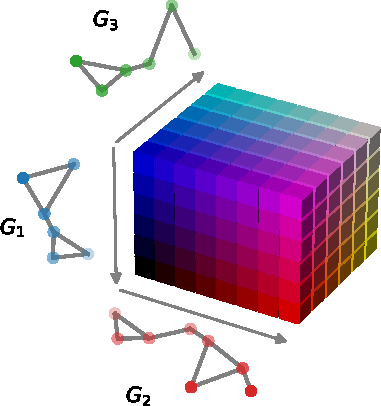
\includegraphics[width=0.4\linewidth]{Figures/coloured_tensor.pdf}
    \end{center}
    \caption[Graphical depiction of an order-3 tensor]{Graphical depiction of an order-3 tensor with graphs underlying each axis}
    \label{fig:3D_colored_tensor}
\end{figure}


In this chapter we extend the methods developed in the previous two chapters, that is Graph Signal Reconstruction (GSR), Kernel Graph Regression (KGR) and Regression with Network Cohesion (RNC), to graphs which are the Cartesian product of three or more factor graphs. 

\begin{itemize}
    \item Summarise chapter aims and output
\end{itemize}




\section{Extending GSP to arbitrary dimensions}

\subsection{The Cartesian product of more than two graphs}

In \cref{sec:graph_products_defined} we gave the general definition of a product between two graphs and highlighted four standard examples, namely the Cartesian, direct, strong and lexicographic products. Each of these product types can be straightforwardly extended to more than two factor graphs by applying their respective definition recursively. For example, consider the Cartesian product between graphs $\mathcal{G}_A = \{\mathcal{V}_A, \mathcal{E}_A\}$, $\mathcal{G}_B = \{\mathcal{V}_B, \mathcal{E}_B\}$ and $\mathcal{G}_C = \{\mathcal{V}_C, \mathcal{E}_C\}$ where $|\mathcal{V}_A| = A$, $|\mathcal{V}_B| = B$ and $|\mathcal{V}_C| = C$. This can be written as 

\begin{equation}
    \mathcal{G} \; = \; \mathcal{G}_A \, \square \; \mathcal{G}_B \, \square \; \mathcal{G}_C \; = \; \{\mathcal{V}, \, \mathcal{E}\}
\end{equation}

The new vertex set, $\mathcal{V}$, is given by the Cartesian product of the individual vertex sets, arranged in lexicographic order. 

\begin{equation}
    \mathcal{V} = \mathcal{V}_A \times \mathcal{V}_B \times \mathcal{V}_C = \{(a, \, b, \, c) \in \mathbb{N}^3 \, | \, a \leq A, \; b \leq B, \text{and} \;  c \leq C\}
\end{equation}

The new edge set, $\mathcal{E}$, is given by recursively applying conditions 1 and 7 from, \cref{sec:graph_products_defined} to the new node set. In particular, any two nodes $(a, \, b, \, c)$ and $(a', b', c')$ are connected in $\mathcal{E}$ if they satisfy any of the following three conditions. 

\vspace{0.5cm}

\begin{table}[h]
    \def\arraystretch{1.5}
    \centering
    \begin{tabular}{lclclc}
        1. & $[a, \, a'] \in \mathcal{E}_A$    & and & $b = b'$  & and & $c = c'$             \\
        2. & $a = a'$    & and & $[b, \, b'] \in \mathcal{E}_B$   & and & $c = c'$             \\
        3. & $a = a'$    & and & $b = b'$  & and & $[c, \, c'] \in \mathcal{E}_C$              \\
    \end{tabular}
\end{table}


\begin{figure}[t]
    \begin{center}
        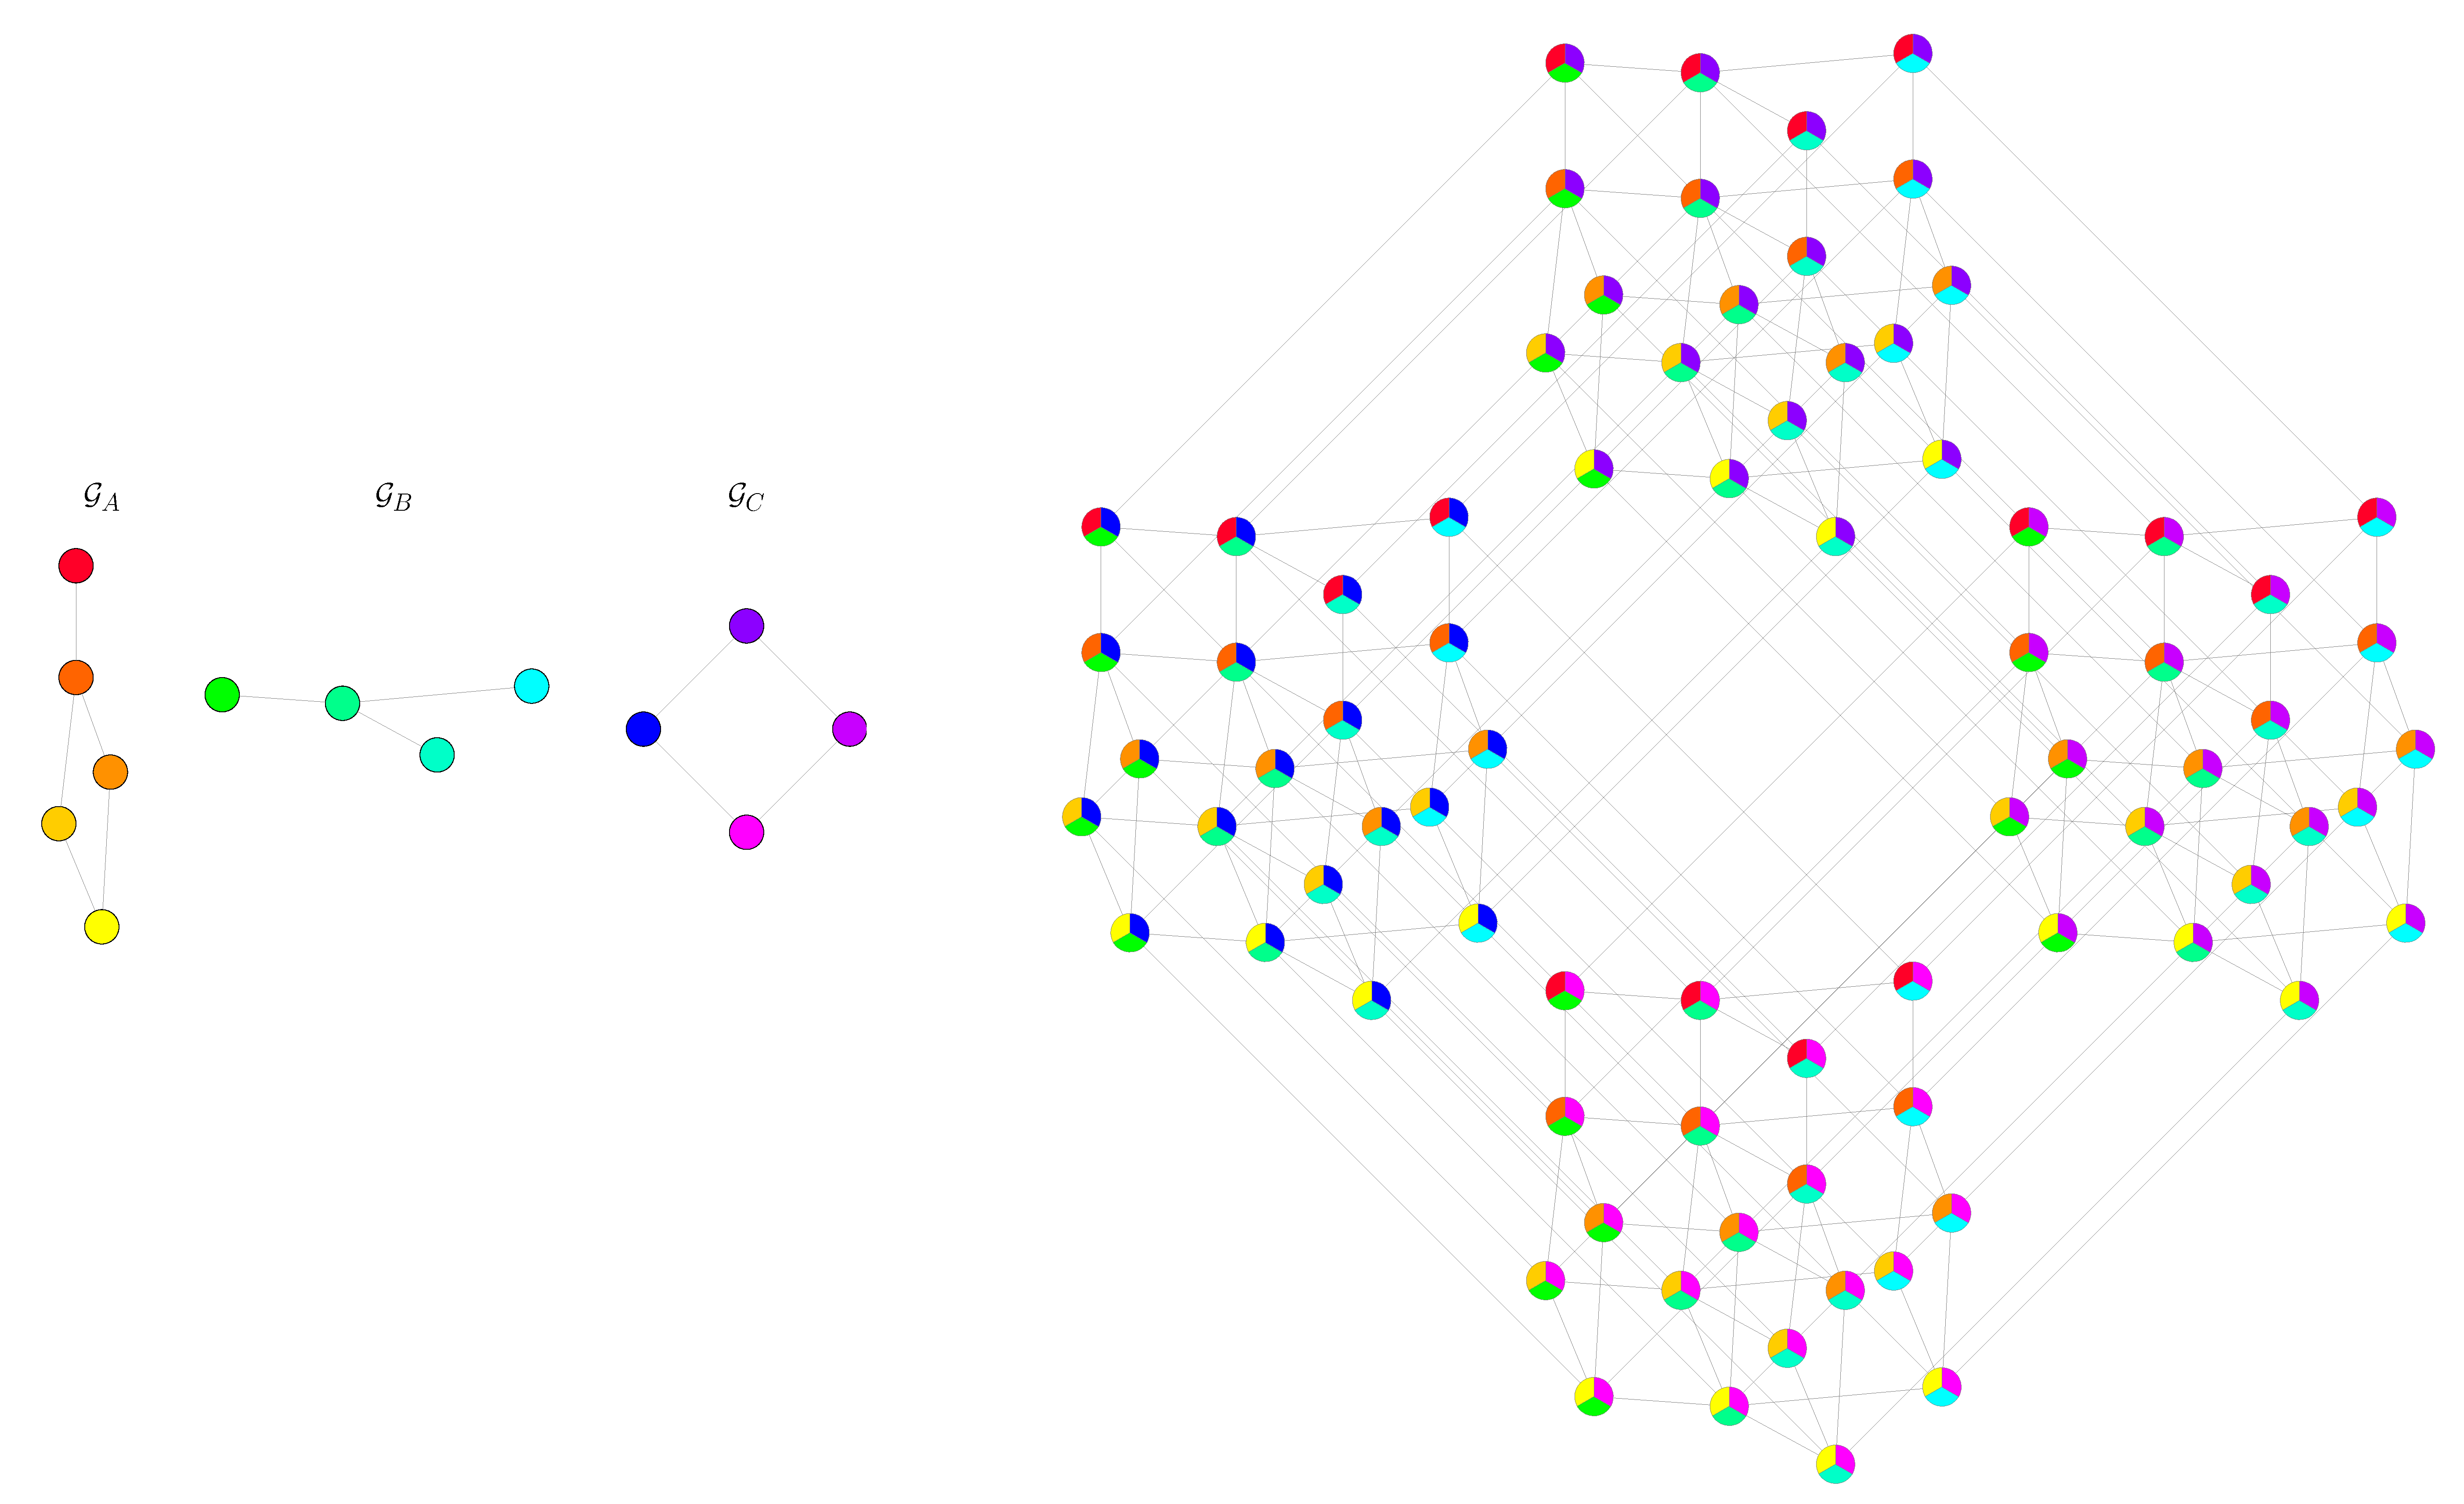
\includegraphics[width=\linewidth]{Figures/3D_CPG.pdf}
    \end{center}
    \caption[Graphical depiction of a 3D Cartesian product graph]{Graphical depiction of a 3D Cartesian product graph}
    \label{fig:3D_CPG}
\end{figure}

\Cref{fig:3D_CPG} gives a visual representation of a Cartesian product graph formed from three simple factor graphs. Notice that the size of the new vertex and edge set both grow very quickly. In particular, 

$$
|\mathcal{V}| = |\mathcal{V}_A| |\mathcal{V}_B| |\mathcal{V}_C| \aand |\mathcal{E}| =  |\mathcal{E}_A| |\mathcal{V}_B| |\mathcal{V}_C| + |\mathcal{V}_A| |\mathcal{E}_B| |\mathcal{V}_C| + |\mathcal{V}_A| |\mathcal{V}_B| |\mathcal{E}_C|
$$

Happily, the adjacency matrix of a Cartesian product graph $\A$ has a straightforward representation in terms of the factor adjacency matrices (here $\A_A$, $\A_B$ and $\A_C$). Specifically, it is given by their Kronecker sum. 

\begin{align}
    \A &= \A_A \oplus \A_B \oplus \A_C \notag \\
    &= \A_A \otimes \I_B \otimes \I_C  + \I_A \otimes \A_B \otimes \I_C + \I_A \otimes \I_B \otimes \A_C
\end{align}

In general, we can consider the Cartesian product of $d$ factor graphs with adjacency matrices denoted as $\A^{(1)} \in \R^{N_1 \times N_2}, \A^{(2)} \in \R^{N_2 \times N_2}, \dots \A^{(d)} \in \R^{N_d \times N_d}$. The full adjacency matrix will have size $N \times N$, where $N = \prod N_i$, and is given by  

\begin{alignat}{4}
    \A = \A^{(1)} & \oplus \A^{(2)} & \oplus \;\; ... \;\; & \oplus \A^{(d)} \notag \\[0.1cm]
    = \A^{(1)} & \otimes \I_{N_2} & \otimes \;\; ... \;\; & \otimes \I_{N_d} +  \notag \\[0.1cm]
    \I_{N_1} & \otimes \A^{(2)} & \otimes \;\; ... \;\; & \otimes \I_{N_d} + \;\; \ldots \;\; +  \notag \\[0.1cm]
    \I_{N_1} & \otimes \I_{N_2} & \otimes \;\; ... \;\; & \otimes \A^{(d)}  
\end{alignat}
    
This can be written compactly as 

\begin{equation}
    \A = \bigoplus_{i=1}^d  \A^{(i)}
\end{equation}

Similarly, the Laplacian of the product graph, $\LL$, can be written as the Kronecker sum of the individual factor graph Laplacians $\LL^{(i)}$. 

\begin{equation}
    \LL = \bigoplus_{i=1}^d  \LL^{(i)}
\end{equation}

We can perform eigendecomposition on each of the individual graph Laplacians as follows. 

\begin{equation}
    \LL^{(i)} = \U^{\,(i)} \LAM^{(i)} (\U^{\,(i)})^\top
\end{equation}

\noindent where $ \U^{(i)}$ is an orthogonal matrix such that each column is an eigenvector of $\LL^{(i)}$, and $\LAM^{(i)}$ is a diagonal matrix containing the corresponding eigenvalues, which are typically listed in ascending order. 

$$
\LAM^{(i)} = 
\begin{bmatrix}
    \lambda_1^{(i)}, &                 &        &                 \\
                     & \lambda_2^{(i)} &        &                 \\
                     &                 & \ddots &                 \\
                     &                 &        & \lambda_{N_i}^{(i)} \\
\end{bmatrix}
$$

Given this, the Laplacian of the product graph can be decomposed as follows. 

\begin{align}
    \LL &= \bigoplus_{i=1}^d \U^{\,(i)} \LAM^{(i)} (\U^{\,(i)})^\top \notag \\[0.2cm]
    &= \left( \bigotimes_{i=1}^d  \U^{\,(i)} \right) \left(\bigoplus_{i=1}^d \LAM^{(i)} \right) \left(\bigotimes_{i=1}^d  \U^{\,(i)} \right)^\top \notag \\[0.2cm]
    &= \U \LAM \U^\top 
\end{align}

\noindent where 

\begin{equation}
    \label{eq:U_LAM_def}
    \U =  \bigotimes_{i=1}^d  \U^{\,(i)} , \quad \text{and} \quad \LAM =  \bigoplus_{i=1}^d \LAM^{(i)}
\end{equation}


Here, we have used the notation $\bigotimes_{i=1}^d  \U^{\,(i)}$ to denote the chained Kronecker product of matrices $\{\U^{\,(i)}  \}$. 

\subsection{Representing \textit{d}-dimensional graph signals}

Since each node in a $d$-dimensional product graph is specified by $d$ independent indices, a signal $\Yt$ existing over the nodes has a natural representation as a tensor of order $d$. One way to conceptualise a $d$-dimensional tensor signal is as a multi-dimensional array with $d$ independent axes. If the $i$-th factor graph has $N_i$ vertices, then $\Yt$ will be of shape $(N_1, \, N_2 , ... N_d)$. An individual element of this tensor signal can be specified via a vector index $\nn = [n_1,\, n_2,\, ...,\, n_d]$, where $1\leq n_i \leq N_i$.

Alternatively, signals can be represented as a vector of length $N = \prod N_i$. This is essential if we are to interpret the $\otimes$ symbol strictly as a Kronecker product, rather than a tensor or outer product. Under the Kronecker interpretation, the chained use of $\otimes$ used in expressions such as \cref{eq:U_LAM_def} results in matrices of shape $N \times N$, providing a linear map from $\R^{N} \rightarrow \R^{N}$. Therefore, for an operator to act on a tensor graph signal $\Yt \in \R^{N_1 \times N_2 \times ... \times N_d}$, we need a method of mapping tensors with shape $(N_1, \, N_2 , ... N_d)$ to vectors of length $N$. In order for this vectorisation process to be consistent with the operators, it should result in a vectors whose elements are arranged in lexicographic order. In some fields, this is referred to as \textit{row-major} vectorisation since, in the case of an order-2 tensor, the index representing the row varies before the column index. In the following, we symbolise this operation mathematically as $\vecrm{\cdot}: \R^{N_1 \times N_2 \times ... \times N_d} \rightarrow \R^N$, and its reverse operation as $\tenrm{\cdot}: \R^N \rightarrow \R^{N_1 \times N_2 \times ... \times N_d}$. We use the `RM' subscript to indicate explicitly that this process is occurring in row-major order, since the standard $\vecc{\cdot}$ function defined for matrices is most commonly assumed to act in column-major order.  

In the following, we use bold lower-case latin symbols (e.g. $\y$) to indicate graph signals existing in their vector form, and bold upper-case calligraphic latin symbols (e.g. $\Yt$) to indicate graph signals in their tensor form. That is, 

\begin{align*}
    \y \in \R^{N} = \vecrm{\Yt}, \quad \implies \quad \Yt \in \R^{N_1 \times N_2 \times ... \times N_d} = \tenrm{\y}
\end{align*}

\Cref{fig:ten_to_vec} shows gives a visual summary of the process of converting between these two representations for an order-3 tensor. 


\begin{figure}[t]
    \begin{center}
        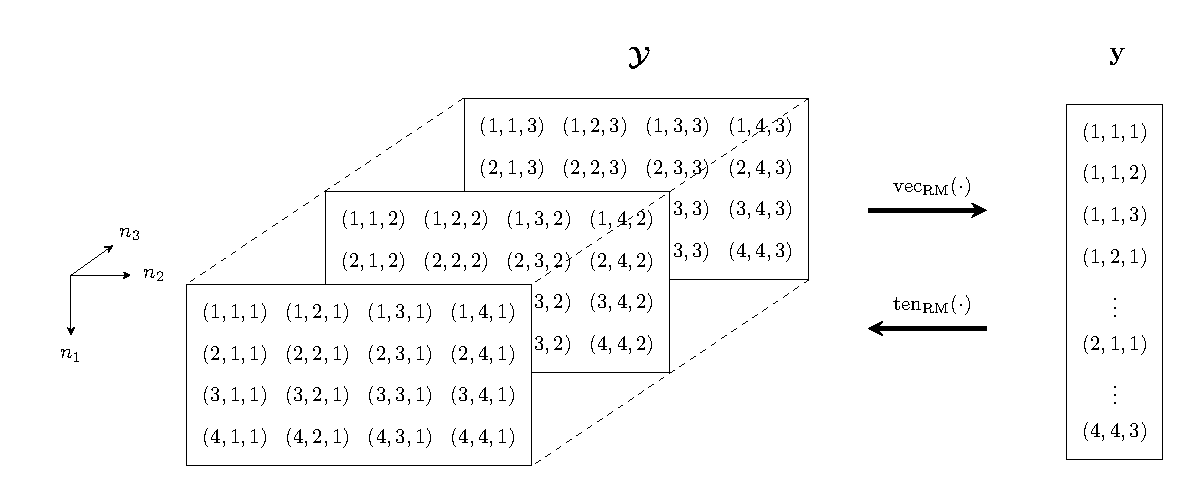
\includegraphics[width=\linewidth]{Figures/Tensor_Digaram.pdf}    
    \end{center}
    \caption[Conversion between a multidimensional array and a vector]{A graphical depiction of the process of converting an order-3 tensor between its multidimensional array and vector form in row-major order. Note that the elements in the vectorised signal are lexicographically ordered. }
    \label{fig:ten_to_vec}
\end{figure}


To calculate the vector index $k$ which a tensor element with index $\nn = [n_1,\, n_2,\, ...,\, n_d]$ is mapped to in row-major order, we can apply the following formula.  

\begin{equation}
    \label{eq:vec}
    k = 1 + \sum_{i=1}^d \Big( \prod_{j=i+1}^d N_j \Big) \, (n_i - 1)
\end{equation}

(Note the $\pm1$ disappear when indexing begins from zero). The reverse operation, i.e. mapping a vector element index $k$ to a tensor index $\nn$ can be achieved by running the algorithm \hyperlink{vectoten}{\textbf{3}}. 


\begin{algorithm}[t]
    \hypertarget{vectoten}{}
    \label{al:vectoten}
    \caption{Mapping a vector element to a tensor element in row major order}
    \begin{algorithmic}
    \vspace{0.15cm}
    \Require{The target vector element $k$} 
    \vspace{0.1cm}
    \Require{The shape of the output tensor $(N_1, N_2, ..., N_d)$} 
    \vspace{0.25cm}
    \State{$k \leftarrow  k - 1$}
    \vspace{0.25cm}
    \For{$i$ \textbf{from} $d$ \textbf{to} 1}
    \vspace{0.25cm}
    \State{$n_i \leftarrow  k \mod N_i$}
    \vspace{0.15cm}
    \State{$k \leftarrow \lfloor k / N_i \rfloor$} 
    \vspace{0.15cm}
    \EndFor
    \vspace{0.25cm}
    \Ensure{$(n_1 + 1, n_2 + 1, ..., n_d + 1)$}
    \end{algorithmic}
\end{algorithm}



Given these two operations, two arrays of any consistent shape can be mapped between one another by first vectorising according to \cref{eq:vec}, and then converting to a tensor using the given algorithm.



\subsection{GSP in \textit{d}-dimensions}



Consider a graph signal $\Yt \in \R^{N_1 \times N_2 \times ... \times N_d}$ represented in its tensor form. In direct analogy to the two dimensional case given in \cref{eq:GFT_2d,eq:IGFT_2d}, we can define the Graph Fourier Transform (GFT) and its corresponding inverse (IGFT) of this signal as follows. 

\begin{alignat}{2}
\label{eq:gft_nd}
    \text{GFT}(\Yt) & = \tenrm{\U^\top \y} && = \tenrm{\left(  \bigotimes_{i=1}^d  \U^{\,(i)} \right)^\top \vecrm{\Yt} } \\
\label{eq:igft_nd}
    \text{IGFT}(\Yt) & = \tenrm{\U \y} && = \tenrm{\left(  \bigotimes_{i=1}^d  \U^{\,(i)} \right) \vecrm{\Yt} }
\end{alignat}

The concept of a graph filter for signals defined on a Cartesian product graph follows naturally from this definition. Just as in the one and two-dimensional case, a graph filter is constructed by first taking the GFT of a signal, then applying some scaling function to each spectral component, then transforming back into the vertex domain via the IGFT. In the simplest case, we can consider an isotropic graph filter function $g(\lambda, \beta)$, such as one of those defined in \cref{tab:iso_filters}. A filter $\HH$, defined to act on a vectorised graph signal, can be represented as an $N \times N$ matrix, constructed as follows. 


\begin{align}
    \label{eq:H_def_dd}
    \HH &= \left( \bigotimes_{i=1}^d  \U^{\,(i)} \right) g\left(\bigoplus_{i=1}^d \LAM^{(i)}; \beta \right) \left(\bigotimes_{i=1}^d  \U^{\,(i)} \right)^\top \notag \\[0.2cm]
        &= \U \, \diag{\vecrm{\Gt}} \, \U^\top
\end{align}


Here, $\Gt$ represents the spectral scaling tensor, which has element $\nn = [n_1,\, n_2,\, ...,\, n_d]$ given by 

\begin{equation}
    \label{eq:Gn_dd1}
    \Gt_{\nn} = g\left(\sum_{i=1}^d \lambda^{(i)}_{n_i}; \, \beta\right)
\end{equation}

In certain special filter types, such as the diffusion filter, this function may be multiplicatively separable. In this case, we have that 

\begin{equation}
    \Gt_{\nn} = \prod_{i=1}^d g\left(\lambda^{(i)}_{n_i}; \, \beta\right)
\end{equation}

This further implies that the graph filter $\HH$ can be decomposed as 

\begin{equation}
    \HH = \bigotimes_{i=1}^d \HH^{(i)}, \where \HH^{(i)} = \U^{(i)} g\left(\LAM^{(i)}\right) \left(\U^{(i)}\right)^\top
\end{equation}

However, in the following, we ignore this special case and assume that the graph filter function is non-separable in general. 

The concept of a multi-way graph filter can be further generalised to include anisotropic filter functions, where the intensity of the filtering operation is not restricted to be equal in each dimension. \Cref{tab:anis_filters} gives some examples of anisotropic graph filter functions defined to act in an arbitrary number of dimensions. Notice how the definition of  

\begin{table}[t]
    \def\arraystretch{1.7}
    \small
    \begin{center}
        \begin{tabular}{|l|c|}
            \hline
            \textbf{Filter}   & $g(\lambdaa; \,\betaa)$                                            \\
            \hline
            1-hop random walk & $(1 + \betaa^\top\lambdaa)^{-1}$                                   \\
            \hline
            Diffusion         & $\exp(-\betaa^\top\lambdaa)$                                       \\
            \hline
            ReLu              & $\max (1 - \betaa^\top\lambdaa, 0)$                                \\
            \hline
            Sigmoid           & $2 \big( 1 + \exp(\betaa^\top\lambdaa)\big)^{-1}$                  \\
            \hline
            Bandlimited       & $1, \,\text{if} \; \betaa^\top\lambdaa \leq 1 \; \text{else} \; 0$ \\
            \hline
        \end{tabular}
    \end{center}
    \caption{Anisotropic graph filter functions in an arbitrary number of dimensions}
    \label{tab:anis_filters}
\end{table}


In this case, the spectral scaling tensor is given by 

\begin{equation}
    \label{eq:Gn_dd2}
    \Gt_{\nn} = g\big(\lambdaa(\nn); \, \betaa\big)
\end{equation}

where $\betaa \in \R^{d}$ is the parameter vector characterising the filter intensity in each dimension, and $\lambdaa(\nn) \in \R^d$ is a vector holding the $n_i$-th eigenvalue of each graph Laplacian in the Cartesian product. 

$$
\lambdaa(\nn) = 
\begin{bmatrix}
    \lambda^{(1)}_{n_1} & \lambda^{(2)}_{n_2} & \dots & \lambda^{(d)}_{n_d}    
\end{bmatrix}^\top
$$

In general, we can define any spectral transformation in tensor terms as follows. 

\begin{equation}
    \Yt' = \text{IGFT} \left( \Gt \circ \text{GFT}(\Yt) \right)
\end{equation}

\subsection{Fast computation of the \textit{d}-dimensional GFT and IGFT}

\label{sec:fast_kron_dd}

Consider the definition of the GFT and IGFT of a $d$-dimensional graph signal given in \cref{eq:gft_nd,eq:igft_nd}. In both cases, we are required to compute the result of a chained Kronecker product matrix acting on a length-$N$ vector. Whilst the obvious approach to computing this product would have time and memory complexity of $O(N^2)$, a much more efficient implementation can be achieved by taking advantage of the Kronecker structure of the matrix. Specifically, the memory and time complexity of this operation can be reduced to $O(N)$ and $O(N\sum N_i)$ respectively. The importance of this fact cannot be understated, as it enables scaling to much larger product graphs that would otherwise be possible. 

This general algorithm for achieving this is well-known, and can be summarised as follows. Consider the application of a chained Kronecker product matrix acting on a vector $\y$. 

$$
\y = \left( \U^{(1)} \otimes \U^{(2)} \otimes ... \otimes \U^{(d)}\right) \z
$$

This can be factorised as follows

$$
\y = \left( \U^{(1)} \otimes \I \otimes ... \otimes \I \right)\left( \I \otimes \U^{(2)} \otimes ... \otimes \I \right) ... \left( \I \otimes \I \otimes ... \otimes \U^{(d)} \right) \z
$$

As is visible, the original multiplication has now been broken into $d$ stages. However, the $i$-th stage can be completed with $N \times N_i$ multiplications by reshaping the vector in the appropriate way and leveraging the properties of the Kronecker product. The reshaping operation can be completed using strided permutation matrices which can be applied in practice for virtually zero computational cost \citep{Granata1992}. This idea is also key to the FFT and related algorithms, which can be understood as finding a recursive Kronecker structure in the Fourier matrix \citep{Tolimieri2013}. 

Work on efficient computational procedures for this operation can be traced back to \cite{Roth1934} who formulated the original 2-dimensional ``vec trick" algorithm. The $d$-dimensional generalisation was proposed in \cite{Pereyra1973} and improved in \cite{DeBoor1979}. More recent work, such as \cite{Fackler2019}, has focused on further optimisations such as minimising data transit times and parallel processing. 

Furthermore, if the $i$-th factor graph in the Cartesian product is a path or ring graph, then the corresponding matrix transformation can be completed with only $N \log N_i$ multiplications by making use of the FCT/FST/FFT algorithms. In the extreme case, where every factor graph has this special structure, the computational complexity reaches parity with the multidimensional FFT algorithm, and will have a runtime complexity of $O(N \log N)$ \citep{Smith1995}. 

In order to execute computations of this nature in a way that is maximally efficient, we have developed the Python library \textit{PyKronecker}, which is described in detail in \cite{Antonian2023}. This library offers a high-level API for constructing Kronecker-based operators and applying them to either vectors or tensors, whilst optimising the underlying computation using parallel GPU processing and Just In Time (JIT) compilation. In the following, it will be assumed that all chained Kronecker product matrices are applied to vectors/tensors using an efficient implementation. This is essential for computing the $d$-dimensional GFT and IGFT, the basic pseudocode for which is shown in algorithm \hyperlink{al:GFT_dd}{\textbf{4}}. Note that the `reshape' operation should always be applied using the row-major convention. This is the standard convention in languages such as C and Python's NumPy library \citep{Harris2020}, but not in languages such as Matlab and Fortran. 

\begin{algorithm}[t]
    \hypertarget{al:GFT_dd}{}
    \label{al:GFT_dd}
    \caption{Efficient GFT and IGFT in $d$-dimensions}
    \begin{algorithmic}
    \vspace{0.25cm}
    \Require{List of Laplacian eigenvector matrices $\left\{\U^{(i)} \in \R^{N_{i} \times N_{i}}\right\}_{i=1}^d$} 
    \vspace{0.8cm}
    \Function{GFT}{$ \Yt \in \R^{N_1 \times N_2 \times ... \times N_d} $}
    \vspace{0.25cm}
    \For{$i$ \textbf{from} 1 \textbf{to} $d$}
    \vspace{0.25cm}
    \State{$\Yt\leftarrow \text{reshape}\Big(\Yt,  \;\big(N_i,\, N / N_i \big) \Big)$}
    \vspace{0.25cm}
    \State{$\Yt \leftarrow \left( \left(\U^{(i)}\right)^\top \; \Yt  \right)^\top$} 
    \vspace{0.25cm}
    \EndFor
    \vspace{0.25cm}
    \State{\textbf{return} $\text{reshape}\Big(\Yt, \; \big(N_1, \, N_2, \; ..., \; N_d \big) \Big)$}
    \vspace{0.25cm}
    \EndFunction
    \vspace{1cm}
    \Function{IGFT}{$ \Zt \in \R^{N_1 \times N_2 \times ... \times N_d} $}
    \vspace{0.25cm}
    \For{$i$ \textbf{from} 1 \textbf{to} $d$}
    \vspace{0.25cm}
    \State{$\Zt\leftarrow \text{reshape}\Big(\Zt,  \;\big(N_i,\, N / N_i \big) \Big)$}
    \vspace{0.25cm}
    \State{$\Zt \leftarrow \left( \U^{(i)} \; \Zt  \right)^\top$} 
    \vspace{0.25cm}
    \EndFor
    \vspace{0.25cm}
    \State{\textbf{return} $\text{reshape}\Big(\Zt, \; \big(N_1, \, N_2, \; ..., \; N_d \big) \Big)$}
    \vspace{0.25cm}
    \EndFunction
    \vspace{0.25cm}
    \end{algorithmic}
\end{algorithm}


\note{A note on tensor notation}{
    The use of tensor algebra is well established in fields such as phyics and mechanics \citep{Renteln2013,Abraham1988}, however, it is less widespread in the signal processing community. For this reason, we choose to adopt a notation that leans more on standard linear algebra, however, all the equations and algorithms discussed in the following chapters could be alternatively written in a purer form of tensor notation. For example, consider the IGFT of a tensor signal $\Zt$. In our notation, this is written as

    \vspace{0.3cm}

    \begin{equation}
        \label{eq:LA_MM}
        \Yt = \text{ten}_{\text{RM}}\left(\left(\bigotimes_{i=1}^d  \U^{\,(i)}\right) \text{vec}_\text{RM}\left(\Zt\right) \right)    
    \end{equation}

    \vspace{0.3cm}

    As is visible, this describes the process in terms of regular matrix-vector multiplication, but requires the additional definition of the $\vecrm{\cdot}$ and $\tenrm{\cdot}$ operations. Alternatively, this expression could be written using tensor indexing and Einstein summation notation as follows. 
    
    \vspace{0.3cm}

    \begin{equation}
    \label{eq:TEN_MM}
    \Yt^{\, i_1, i_2, ..., i_d} = \left(\U^{(1)}\right)^{i_1}_{j_1}\left(\U^{(2)}\right)^{i_2}_{j_2} ... \left(\U^{(d)}\right)^{i_d}_{j_d} \, \Zt^{\, j_1, j_2, ..., j_d}
    \end{equation}

    \vspace{0.3cm}

    Note that here the indices $j_1, j_2, ..., j_d$ on the right hand side are implicitly summed over. This eliminates the need to consider vectorisation at all and is perhaps a more elegant way of describing the $d$-dimensional GFT/IGFT. However, there are multiple indices to keep track of which becomes somewhat unaesthetic in a variable number of dimensions.

    \vspace{0.3cm}
    
    Both forms offer different trade-offs, however, there is no practical difference when it comes to executing the signal precessing algorithms themselves. Note that, as described in \cref{sec:fast_kron_dd}, the full $N \times N$ matrix implied by \cref{eq:LA_MM} is never actually instantiated in memory (see algorithm \hyperlink{KronMatMul}{\textbf{4}}).

}

\section{Tensor Graph Signal reconstruction}

The model we use to describe graph signal reconstruction in the multi-dimensional setting is as follows. Consider a tensor signal $\Yt$ of shape $\big(N_1, \, N_2, \, ... \, N_d \big)$ with elements interpreted as existing on the nodes of a $d$-dimensional Cartesian product graph. Only a partial set $\mathcal{S} = \{\nn_1, \, \nn_2, \, ... \}$ of the vector elements of $\Yt$ are available at observation time, with unobserved values set to zero. The goal is to estimate the signal value at these unobserved entries. 

The binary sensing tensor $\St$, of the same shape as $\Yt$, indicates which elements of $\Yt$ were observed in the following way 

\begin{equation}
    \St_{\nn} = \begin{cases}
        1 & \text{if} \;\; \nn \in \mathcal{S} \\
        0 & \text{otherwise}
    \end{cases}
\end{equation}

In analogy with the two dimensional case, (see \cref{sec:problem_statement_2d}), we assume that $\Yt$ is a noisy partial observation of an underlying tensor $\Ft$ which is smooth with respect to the topology of the Cartesian product graph. This is represented in the following statistical model. 

\begin{equation}
    \Yt = \St \circ \big(\Ft + \Et \big)
\end{equation}

where, here, the $\circ$ symbol represents the generalised tensor Hadamard product, i.e. element-wise multiplication of two tensors. $\Et$ is a random tensor where each element has an independent normal distribution with with unit variance. That is,

\begin{equation}
    \vecrm{\Et} \, \sim \, \mathcal{N}(\mathbf{0}, \, \I)
\end{equation}

Given this distribution over the model noise, the conditional distribution of $\Yt |  \Ft$ is given by 

\begin{equation}
    \vecrm{\Yt} \, | \, \vecrm{\Ft} \, \sim \, \mathcal{N}\Big(\vecrm{\St \circ \Ft}, \; \diag{\vecrm{\St}}\Big)
\end{equation}

Or, more concisely, 

\begin{equation}
    \y \, | \, \f \, \sim \, \mathcal{N}\big(\s \circ \f, \; \D_{\St} \big)
\end{equation}

where $\D_{\St} = \diag{\s}$. In order to encode the belief that the underlying tensor $\Ft$ is smooth with respect to the topology of the graph, we can make use of the following prior distribution. 

\begin{equation}
    \f \, \sim \, \mathcal{N}\left( \mathbf{0}, \, \gamma^{-1} \HH^2 \right) 
\end{equation}

where $\HH$ is constructed from a graph filter function in the manner specified in \cref{eq:H_def_dd}. The intuition for this prior can be obtained from a direct generalisation of the one and two dimensional cases. In essence, tensor signals drawn from this prior will have the same probability density function as iid noise filtered by $\HH$, so samples will be naturally smooth with respect to the topology of the underlying Cartesian product graph. By applying Bayes theorem, we obtain the posterior distribution for $\f$ conditioned on $\y$. 


\begin{equation}
    \f \, | \, \y \sim \Norm{\PP^{-1} \y}{\PP^{-1}}
\end{equation}

where 

\begin{equation}
    \PP = \D_{\St} + \gamma \HH^{-2}
\end{equation}

Therefore, the mean of this posterior is obtained by solving the following linear system.

\begin{equation}
    \label{eq:lin_system_dd}
    \f^{\star} = \left(\D_\St + \gamma \HH^{-2}\right)^{-1} \y
\end{equation}

Once again, we are faced with a similar set of problems to those outlined in \cref{sec:problem_statement_2d}. Namely, the coefficient matrix is very large and potentially ill-defined. This can be solved by turing to iterative methods such as the SIM and CGM, which are repeated here in their form adapted for the general tensor case. 

\subsection{Tensor SIM}

Generalising the SIM, which we describe in \cref{sec:SIM}, to the tensor setting is straightforward. In particular, \cref{eq:lin_system_dd} can be solved by splitting the coefficient matrix $\left(\D_\St + \gamma \HH^{-2}\right)$ into $\M - \N$, where $\M$ and $\N$ take on the following values
 
\begin{equation}
    \M = \gamma \HH^{-2} + \I, \aand \N = \D_{\St'}
\end{equation}

where $\D_{\St'} = \diag{\mathbf{1} - \vecrm{\St}}$. In this case, the inverse of $\M$ has the form 


\begin{align}
\M^{-1} &= \left( \bigotimes_{i=1}^d  \U^{\,(i)} \right) \, \diag{\vecrm{\Jt}}\, \left(\bigotimes_{i=1}^d  \U^{\,(i)} \right)^\top \notag \\[0.2cm]
&= \U \, \D_\Jt \, \U^\top
\end{align}

where the tensor $\Jt$ has entries with the vector index $\nn = [n_1,\, n_2,\, ...,\, n_d]$ given by 

\begin{equation}
    \Jt_{\nn} = \frac{\Gt_{\nn}^2}{\Gt_{\nn}^2 + \gamma}.
\end{equation}

Here, the entries of $\Gt$ are given by either \cref{eq:Gn_dd1} or \cref{eq:Gn_dd2}, which correspond to an isotropic or anisotropic filter function respectively. In a very similar manner to \cref{eq:sim_update}, the SIM update equation is given by 

\begin{equation}
    \label{eq:sim_update_dd}
    \f_{k+1} = \M^{-1}\N \f_{k} + \M^{-1} \y
\end{equation}

Note that each step can be achieved with time complexity $O(N \sum N_i)$ by making use of the fast Kronecker algorithm for computing the $d$-dimensional GFT/IFGT highlighted in \cref{sec:fast_kron_dd}. To be explicit, this update formula can be computed efficiently as 

\begin{align*}
    \Ft_{k+1} &= \text{IGFT} \Big( \Jt \circ \text{GFT}\big(\St' \circ \Ft_{k}\big)\Big)  + \Ft_{0} \\[0.2cm]
    \text{where} \quad \Ft_{0} &= \text{IGFT} \Big( \Jt \circ \text{GFT}\big(\Yt \big)\Big) 
\end{align*}

or, equivalently,

\begin{align*}
    \Delta \Ft_{k+1} &= \text{IGFT}  \Big( \Jt \circ \text{GFT}\big(\St' \circ \Delta \Ft_{k}\big)\Big)  \\[0.2cm]
    \text{where} \quad \Delta \Ft_{0} &= \text{IGFT} \Big( \Jt \circ \text{GFT}\big(\Yt \big)\Big)  
\end{align*}

using the fast GFT/IGFT algorithms described in \hyperlink{al:GFT_dd}{\textbf{4}}. For clarity, the full SIM algorithm is given in algorithm \hyperlink{al:SIM_dd}{\textbf{5}}. 

\begin{algorithm}[t]
    \hypertarget{al:SIM_dd}{}
    \caption{The tensor SIM for GSR}
    \begin{algorithmic}
        \vspace{0.15cm}
        \Require{Observation tensor $\Yt \in \R^{N_1 \times N_2 \times ... \times N_d}$}
        \vspace{0.15cm}
        \Require{Sensing tensor $\St \in [0, 1]^{N_1 \times N_2 \times ... \times N_d}$}
        \vspace{0.15cm}
        \Require{Factor graph Laplacians $\{\LL^{(i)} \in \R^{N_i \times N_i}\}_{i=1}^d $}
        \vspace{0.15cm}
        \Require{Regularisation parameter $\gamma \in \R^{+}$}
        \vspace{0.15cm}
        \Require{Graph filter function $g(\, \cdot\, \,; \betaa \in \R^{d})$}
        \vspace{0.5cm}
        \State{For $i$ from 1 to $d$, decompose $\LL^{(i)}$ into $\U^{(i)} \LAM^{(i)} \left(\U^{(i)}\right)^\top$}
        \vspace{0.15cm}
        \State{Initialise $\Gt, \Jt, \St'$}
        \vspace{0.5cm}
        \For{$n_1$ \textbf{from} 1 \textbf{to} $N_1$}
        \For{$n_2$ \textbf{from} 1 \textbf{to} $N_2$} \\
        \hspace*{0.7cm} $\ddots$
        \For{$n_d$ \textbf{from} 1 \textbf{to} $N_d$}
        \vspace{0.25cm}
        \State{$\nn \leftarrow [n_1, n_2, ..., n_d]$}
        \vspace{0.15cm}
        \State{$\Gt_{\nn} \leftarrow g\big(\lambdaa(\nn); \, \betaa\big)$ }
        \vspace{0.15cm}
        \State{$\Jt_{\nn} \leftarrow \Gt_{\nn}^2 \, / \, (\Gt_{\nn}^2 + \gamma)$ }
        \vspace{0.15cm}
        \State{$\St_{\nn}' \leftarrow 1 - \St_\nn$}
        \vspace{0.25cm}
        \EndFor
        \EndFor \\
        \hspace*{0.1cm} \reflectbox{$\ddots$}
        \EndFor
        \vspace{0.5cm}
        \State{$\Delta\Ft \leftarrow \text{IGFT}  \Big( \Jt \circ \text{GFT}\big( \Yt \big)\Big) $}
        \vspace{0.15cm}
        \State{$ \Ft  \leftarrow \Delta\Ft$}
        \vspace{0.15cm}
        \While{$|\Delta\Ft| > \text{tol}$}
        \vspace{0.15cm}
        \State{$\Delta\Ft \leftarrow \text{IGFT} \Big( \Jt \circ \text{GFT}\big(\St' \circ \Delta \Ft_{k} \big)\Big) $}
        \vspace{0.15cm}
        \State{$ \Ft \leftarrow  \Ft  + \Delta\Ft$}
        \vspace{0.15cm}
        \EndWhile
        \vspace{0.5cm}
        \Ensure{$ \Ft $}
        \vspace{0.15cm}
        \label{al:SIM_dd}
    \end{algorithmic}
\end{algorithm}

Once again, the worst-case scaling rate of the number of steps required for convergence, $n_{\text{SIM}}$, is bounded by

$$
\frac{1}{\log(1 + \gamma) - \log m} \; \leq \; n_{\text{SIM}} \; \leq \; \frac{1}{\log(1 + \gamma)}
$$

where $m$ is the fraction of data that is missing in the input tensor $\Yt$ (see \cref{sec:convergence}). As before, the true scaling rate will depend on the strength of the graph filter. 

\subsection{Tensor CGM}

The tensor version of the CGM also follows naturally from the two-dimensional case outlined in \cref{sec:CGM}. In particular, \cref{eq:lin_system_dd} can be transformed into the following equivalent preconditioned linear system. 

\begin{equation}
    \label{eq:lin_system_precon_dd}
    \f^{\star} = \PHI \left( \PHI^\top \left(\D_\St + \gamma \HH^{-2}\right)\PHI \right)^{-1}\PHI^\top \y
\end{equation}

where, in the tensor case, 

\begin{equation}
    \PHI = \left( \bigotimes_{i=1}^d  \U^{\,(i)} \right) \, \diag{\vecrm{\Gt}} = \U \D_\Gt
\end{equation}

This means \cref{eq:lin_system_precon_dd} can be expressed as 

\begin{equation}
    \f^{\star} = \PHI \left( \D_\Gt \U^\top \D_\St \U \D_\Gt + \gamma \I_N \right)^{-1}\PHI^\top \y
\end{equation}

Note that, once again, this preconditioned coefficient matrix can be multiplied onto any appropriate tensor $\Zt$ efficiently by making use of the chained Kronecker multiplication procedure given in algorithm \hyperlink{KronMatMul}{\textbf{4}}. As with the SIM, this can be performed with $O(N \sum N_i)$ multiplications. In particular, 

\begin{align*}
    \Zt' &= \tenrm{\big( \D_\Gt \U^\top \D_\St \U \D_\Gt + \gamma \I \big) \vecrm{\Zt}} \\[0.2cm]
    &= \Gt \circ \text{GFT} \Big( \St \circ \text{IGFT} \big(\Gt \circ \Zt\big) \Big)  + \gamma \Zt
\end{align*}


\begin{algorithm}[t]
    \hypertarget{al:CGM_dd}{}
    \caption{The tensor CGM for GSR}
    \begin{algorithmic}
        \vspace{0.15cm}
        \Require{Observation tensor $\Yt \in \R^{N_1 \times N_2 \times ... \times N_d}$}
        \vspace{0.15cm}
        \Require{Sensing tensor $\St \in [0, 1]^{N_1 \times N_2 \times ... \times N_d}$}
        \vspace{0.15cm}
        \Require{Factor graph Laplacians $\{\LL^{(i)} \in \R^{N_i \times N_i}\}_{i=1}^d $}
        \vspace{0.15cm}
        \Require{Regularisation parameter $\gamma \in \R^{+}$}
        \vspace{0.15cm}
        \Require{Graph filter function $g(\, \cdot\, \,; \betaa \in \R^{d})$}
        \vspace{0.5cm}
        \State{For $i$ from 1 to $d$, decompose $\LL^{(i)}$ into $\U^{(i)} \LAM^{(i)} \left(\U^{(i)}\right)^\top$}
        \vspace{0.15cm}
        \State{Initialise $\Gt'$}
        \vspace{0.5cm}
        \For{$n_1$ \textbf{from} 1 \textbf{to} $N_1$}
        \For{$n_2$ \textbf{from} 1 \textbf{to} $N_2$} \\
        \hspace*{0.7cm} $\ddots$
        \For{$n_d$ \textbf{from} 1 \textbf{to} $N_d$}
        \vspace{0.25cm}
        \State{$\nn \leftarrow [n_1, n_2, ..., n_d]$}
        \vspace{0.15cm}
        \State{$\Gt_{\nn} \leftarrow g\big(\lambdaa(\nn); \, \betaa\big)$ }
        \vspace{0.25cm}
        \EndFor
        \EndFor \\
        \hspace*{0.1cm} \reflectbox{$\ddots$}
        \EndFor
        \vspace{0.5cm}
        \State{Initialise $\Zt$}
        \vspace{0.15cm}
        \State{$\Rt \leftarrow \Gt \circ \text{GFT} \left( \Yt \right)$}
        \vspace{0.15cm}
        \State{$\Dt \leftarrow \Rt$}
        \vspace{0.5cm}
        \While{$|\Delta\RR| > \text{tol}$}
        \vspace{0.25cm}
        \State{$\At \leftarrow \Gt \circ \text{GFT} \Big( \St \circ \text{IGFT} \big(\Gt \circ \Dt \big) \Big)  + \gamma \Dt  $}
        \vspace{0.15cm}
        \State{$\alpha \leftarrow  \sum_{\nn} \Rt_{\nn}^2 \, / \, \sum_{\nn} \Rt_\nn \At_\nn $}
        \vspace{0.15cm}
        \State{$\Zt \leftarrow  \Zt + \alpha \Dt $}
        \vspace{0.15cm}
        \State{$\Rt \leftarrow  \Rt - \alpha \At $}
        \vspace{0.15cm}
        \State{$\delta \leftarrow \sum_{\nn} \Rt_{\nn}^2  \, / \, \sum_{\nn} (\Rt + \alpha \At)^2$}
        \vspace{0.15cm}
        \State{$\Dt \leftarrow  \Rt + \delta \Dt $}
        \vspace{0.25cm}
        \EndWhile
        \vspace{0.5cm}
        \Ensure{$\text{IGFT} \left(  \Gt \circ \Zt \right)$}
        \vspace{0.15cm}
    \end{algorithmic}
    \label{al:CGM_dd}
\end{algorithm}



Just as with the two-dimensional case, we can bound the condition number of the preconditioned coefficient matrix to find the worst case scaling rates in the limit of a weak and strong filter. As before, this falls between

$$
\sqrt{\frac{1 - m + \gamma}{\gamma}} \; \leq \; n_{\text{CGM}} \; \leq \; \sqrt{\frac{1+\gamma}{\gamma}}
$$

\section{Kernel Graph Tensor Regression}

Hello

\section{Tensor Regression with Network Cohesion}

Ahhhh

